\documentclass{beamer}
\usepackage{amsmath,amssymb,amsthm,slashed, euscript}
\usepackage{mathrsfs} 

\usepackage{tikz}
\usepackage{tikz-cd}

%\usepackage{mathtools}

\usetikzlibrary{matrix}
\usetikzlibrary{cd}


\textwidth=110mm


\title{Hurewicz homomorphism of $C^*$-algebras}
\institute
{
 Noncommutative geometry and topology
}

\author{Petr R. Ivankov  }



\theoremstyle{plain}
\newtheorem{empt}{}
\newtheorem{defn}{Definition}
\newtheorem{rem}{Remark}
\newtheorem{exm}{Example}
\newtheorem*{claim}{Claim}
\newtheorem{prop}{Proposition}
\newtheorem{lem}{Lemma}%[section]
\newtheorem{thm}{Theorem}%[section]



\newcommand{\A}{\mathcal{A}}
\newcommand{\be}{\begin{equation}}
\newcommand{\ee}{\end{equation}}
\newcommand{\Ga}{\Gamma}
\newcommand{\B}{\mathcal{B}}
\newcommand{\Cc}{\mathcal{C}}
\newcommand{\C}{\mathbb{C}}
\newcommand{\D}{\mathcal{D}}
\newcommand{\G}{\mathcal{G}}
\newcommand{\Hc}{\mathcal{H}}
\newcommand{\Lc}{\mathcal{L}}
\newcommand{\Pc}{\mathcal{P}}
\newcommand{\Sc}{\mathcal{S}}
\newcommand{\U}{\mathcal{U}}
\newcommand{\rar}{\rightarrow}
\newcommand{\Ef}{\mathbb{E}}
\newcommand{\desc}{\mathfrak{desc}}

\newcommand{\ga}{\gamma} 
%Uppercase Gothic characters
\newcommand{\gtA}{\mathfrak{A}}
\newcommand{\gtB}{\mathfrak{B}}
\newcommand{\gtM}{\mathfrak{M}}
\newcommand{\gtN}{\mathfrak{N}}
\newcommand{\gtP}{\mathfrak{P}}
\newcommand{\gtS}{\mathfrak{S}}
\newcommand{\K}{\mathcal{K}}

%Lowercase Gothic characters
\newcommand{\gtf}{\mathfrak{f}}
\newcommand{\gtg}{\mathfrak{g}}
	\newcommand{\End}{\mathrm{End}}       %%

%Bold Characters
\newcommand{\Cb}{\mathbb{C}}
\newcommand{\Nb}{\mathbb{N}}
\newcommand{\Rb}{\mathbb{R}}
\newcommand{\Zb}{\mathbb{Z}}

%Uppercase Greek characters
\newcommand{\Gm}{\Gamma}
\newcommand{\Te}{\Theta}
\newcommand{\Om}{\Omega}
\newcommand{\s}{ }

%Lowercase Greek characters
\newcommand{\al}{\alpha}
\newcommand{\gm}{\gamma}
\newcommand{\dl}{\delta}
\newcommand{\sg}{\sigma}
\newcommand{\ph}{\varphi}
\newcommand{\te}{\theta}
\newcommand{\ze}{\zeta}
\newcommand{\lift}{\mathfrak{lift}}
\newcommand{\eps}{\varepsilon}                    %% tensor product


\newcommand{\Id}{\mathrm{Id}}
\newcommand{\Aut}{\mathrm{Aut}}
\newcommand{\Coo}{{\mathrm{C}}^\infty}
\newcommand{\alg}{\mathrm{alg}}
\newcommand{\diag}{\mathrm{diag}}
\newcommand{\spinc}{\textbf{$spin^c$}}
\newcommand{\Hom}{\mathrm{Hom}}
\newcommand{\supp}{\mathrm{supp}}
\newcommand{\Ccl}{\mathbf{C}l}
\newcommand{\xto}{\xrightarrow}
\newcommand{\T}{\mathbb{T}} 
\newcommand{\lto}{\longrightarrow}
\newcommand{\ox}{\otimes}
\newcommand{\nb}{\nabla}
\newcommand{\sS}{\mathcal{S}}
\newcommand{\Dn}{D\!\!\!\!/}
%\newcommand{\ij}{{i,j}}
\newcommand{\aC}{\ensuremath{\underline{\Cb}} }
\newcommand{\scp}[2]{\left\langle{#1},{#2}\right\rangle}
\newcommand{\op}[1]{J{#1}J^\dag}
\newcommand{\sA}{\mathcal{A}} 
\newcommand{\sB}{\mathcal{B}}       %%
\newcommand{\sC}{\mathcal{C}}       %%
\newcommand{\sD}{\mathcal{D}}       %%
\newcommand{\sE}{\mathcal{E}}       %%
\newcommand{\sF}{\mathcal{F}}       %%
\newcommand{\sG}{\mathcal{G}}       %%
\newcommand{\sH}{\mathcal{H}}       %%
\newcommand{\sI}{\mathcal{I}}       %%
\newcommand{\sJ}{\mathcal{J}}       %%
\newcommand{\sK}{\mathcal{K}}       %%
\newcommand{\sL}{\mathcal{L}}       %%
\newcommand{\sM}{\mathcal{M}}       %%
\newcommand{\sN}{\mathcal{N}}       %%
\newcommand{\sO}{\mathcal{O}}       %%
\newcommand{\sP}{\mathcal{P}}       %%
\newcommand{\sQ}{\mathcal{Q}}       %%
\newcommand{\sR}{\mathcal{R}}       %%
\newcommand{\sT}{\mathcal{T}}       %%
\newcommand{\sU}{\mathcal{U}}       %%
\newcommand{\sV}{\mathcal{V}}       %%
\newcommand{\sX}{\mathcal{X}}       %%
\newcommand{\sY}{\mathcal{Y}}       %%
\newcommand{\sZ}{\mathcal{Z}}       %%
\newcommand{\N}{\mathbb{N}}                  %% 

\renewcommand{\a}{\alpha}     
\newcommand{\la}{\lambda}     
\newcommand{\La}{\Lambda}
\newcommand{\bt}{\beta}           %% short for  \beta
 \renewcommand{\H}{\mathcal{H}}               %% Hilbert space
 
 	\newcommand{\bean}{\begin{eqnarray*}}
 	\newcommand{\eean}{\end{eqnarray*}}
    
\newcommand{\bydef}{\stackrel{\mathrm{def}}{=}}  
\newcommand{\hookto}{\hookrightarrow}        %% abbreviation
  \usepackage{graphicx}
  \graphicspath{ {./images/} }
  \usepackage{tikz}
\usetikzlibrary{calc,trees,positioning,arrows,chains,shapes.geometric,%
	decorations.pathreplacing,decorations.pathmorphing,shapes,%
	matrix,shapes.symbols}
	
	\usetikzlibrary{trees,positioning,shapes,shadows,arrows}
  

\tikzset{
	basic/.style  = {draw, text width=2cm, drop shadow, font=\sffamily,     rectangle},
	root/.style   = {basic, rounded corners=2pt, thin, align=center,
		fill=green!30},
	level 2/.style = {basic, rounded corners=6pt, thin,align=center,     fill=green!60,
		text width=8em},
	level 3/.style = {basic, thin, align=left, fill=pink!60, text width=6.5em}
}
\begin{document}
%\titlepage
\begin{frame}
  \titlepage
\end{frame}


\section{Coverings of $C^*$-algebras}
\begin{frame}
\centering	\huge	Coverings of $C^*$-algebras\normalsize
	
	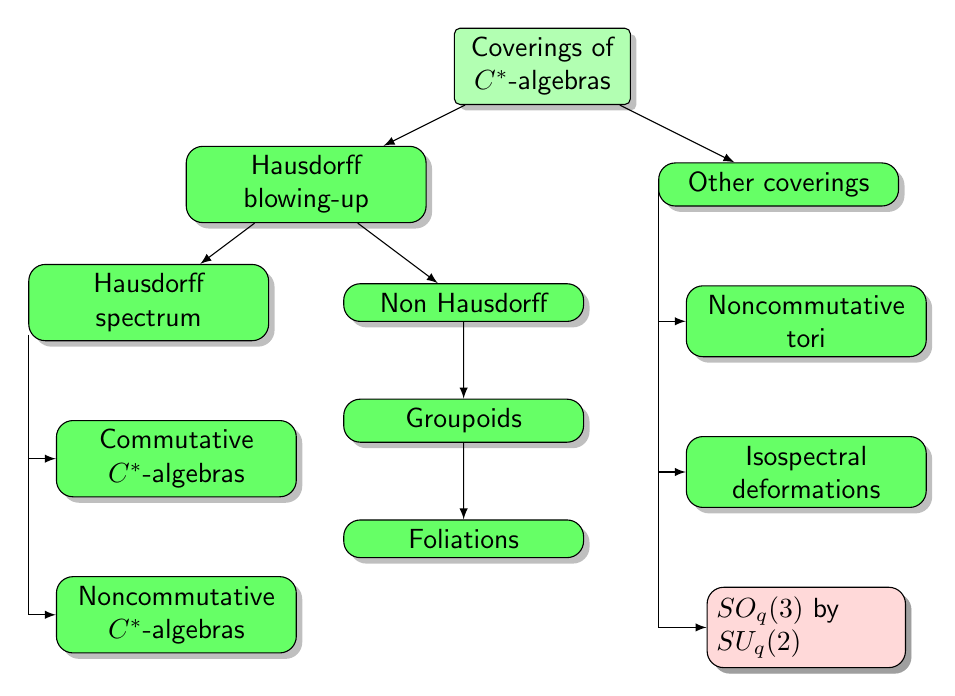
\begin{tikzpicture}[
		level 1/.style={sibling distance=60mm},
		level 2/.append style={sibling distance=40mm},
		edge from parent/.style={->,draw},
		>=latex]
		
		% root of the the initial tree, level 1
		\node[root] {Coverings of $C^*$-algebras}
		% The first level, as children of the initial tree
		child {node[level 2] (ch1) {Hausdorff blowing-up}
			child {node[level 2] (c1) {Hausdorff spectrum}}
			child {node[level 2] (c2) {Non Hausdorff}}{
				child {node[level 2] (c3) {Groupoids}}{
					child {node[level 2] (c4) {Foliations}}
				}
			}
		}
		child {node[level 2] (ch2) {Other coverings}
		};
		\begin{scope}[every node/.style={level 2}]
			\node [below = of  ch2, xshift=10pt] (ch21) {Noncommutative tori};
			\node [below = of  ch21] (ch22) {Isospectral deformations};
			\node [level 3] [below = of  ch22]  (ch23) {$SO_q(3)$ by $SU_q(2)$};
		\end{scope}	
		\begin{scope}[every node/.style={level 2}]
			\node [below = of  c1, xshift=10pt] (c11) {Commutative $C^*$-algebras};
			\node [below = of  c11] (c12) {Noncommutative $C^*$-algebras};
		\end{scope}	
		\foreach \value in {1,...,2}
		\draw[->] (c1.195) |- (c1\value.west);	
		\foreach \value in {1,...,3}
		\draw[->] (ch2.180) |- (ch2\value.west);
	\end{tikzpicture}	
	
\end{frame}
\section{Finite-fold coverings}
\begin{frame}
	\begin{center}
	\huge{Finite-fold coverings}
	\end{center}
	\begin{theorem} 	\alert{Alexander Pavlov, Evgenij Troitsky}.
		Suppose both $\mathcal X$ and $\mathcal Y$ are compact Hausdorff connected spaces and $p :\mathcal  Y \to \mathcal X$
		is a continuous surjection. If $C(\mathcal Y )$ is a projective finitely generated Hilbert module over
		$C(\mathcal X)$ with respect to the action
		\begin{equation*}
			(f\xi)(y) = f(y)\xi(p(y)), ~ f \in  C(\mathcal Y ), ~ \xi \in  C(\mathcal X),
		\end{equation*}
		then $p$ is a finite-fold  covering.
	\end{theorem}
	It is naturally to define a finite-fold covering of $C^*$-algebras as an injective $*$-homomorphisms $A\hookto \widetilde A$ such that $ \widetilde A$-is a finitely generated Hilbert module over
	$A$. However this definition does not gives good generalizations of results  related to topological coverings.
	
\end{frame}
\begin{frame}
  \begin{definition}\label{connected_c_a_defn}
	We say that a $C^*$-algebra $A$ is \alert{connected} if it cannot be represented as a direct sum  $A \cong A' \oplus A''$ of nontrivial $C^*$-algebras $A'$ and $A''$.
	
	% (the Gelfand spectrum of the center of $M\left( A\right) $ is connected). Let $A \subset B$ be a connected subalgebra. We say that $A$ is a \alert{connected component} of $B$ if  $1_{M\left( A\right) }$ lies in the center of $1_{M\left( B\right) }$.
\end{definition}
\begin{definition}\label{connected_comp_defn}
	A connected closed two-sided ideal $A$ of  $C^*$-algebra $B$ is said to be a \alert{connected component of}  $B$ is there is a direct sum $B = A \oplus A'$ of $C^*$-algebras.
	\end{definition}
\end{frame}
\begin{frame}
   \begin{definition}\label{fin_quasi_defn}
	Let both  $A$ and  $\widetilde{A}$ are connected $C^*$-algebras, and let $\pi: A \hookto \widetilde{A}$ be an injective $*$-homomorphism of % connected	  
	$C^*$-algebras. Let $G$ be a finite  group of *-automorphisms of $\widetilde{A}$ such that 	$\pi\left(A\right) = \widetilde{A}^G\stackrel{\text{def}}{=}\left\{
	\left.a\in \widetilde{A}~\right|~ a = g a;~ \forall g \in G\right\}$.	We say that the triple $\left(A, \widetilde{A}, G \right)$ and/or the quadruple $\left(A, \widetilde{A}, G, \pi \right)$ and/or $*$-homomorphism $\pi: A \hookto \widetilde{A}$   is a \alert{noncommutative finite-fold  quasi-covering}. We write
	\be\label{fin_cov_gr_eqn}
	G\left(\left.\widetilde{A}~\right| {A} \right) \stackrel{\text{def}}{=}  	G.
	\ee
\end{definition}
\end{frame}
\begin{frame}
	\begin{definition}\label{pre_defn} \alert{Pet Ivankov}.
		Let $\pi: A \hookto \widetilde{A}$ be an injective *-homomorphism of connected  $C^*$-algebras such that following conditions hold:
		\begin{enumerate}
			\item[(a)] If $\Aut\left(\widetilde{A} \right)$ is a group of *-automorphisms of $\widetilde{A}$ then the group  
			$
			G \bydef \left\{ \left.g \in \Aut\left(\widetilde{A} \right)~\right|~ g\pi\left( a\right)  = \pi\left( a\right) ;~~\forall a \in A\right\}
			$
			is finite.
			\item[(b)] 	\be\label{cond_b_eqn}
			\pi\left( 	A\right)  = \widetilde{A}^G\stackrel{\text{def}}{=}\left\{\left.a\in \widetilde{A}~~\right|~ a = g a;~ \forall g \in G\right\}.\ee
		\end{enumerate}
		We say that the quadruple $\left(A, \widetilde{A}, G, \pi \right)$ and/or *-homomorphism $\pi: A \to \widetilde{A}$   is a \alert{noncommutative finite-fold  pre-covering}. 
	\end{definition}
	
\end{frame}
\begin{frame}
	\begin{definition}
		\alert{Petr Ivankov}
		Let $\left(A, \widetilde{A}, G, \pi \right)$ be a  noncommutative finite-fold  pre-covering. Suppose both $A$ and  $\widetilde{A}$ are unital. We say that $\left(A, \widetilde{A}, G, \pi \right)$ is an \alert{unital noncommutative finite-fold  covering} if $\widetilde{A}$ is a finitely generated projective  $A$-module.
	\end{definition}
	\begin{lemma}
		\alert{Petr Ivankov, Alexander Pavlov, Evgenij Troitsky.}
		If $\mathcal  X$ is a connected, compact, Hausdorff space then there is a natural 1-1 correspondence 
		$$
		\left(p:\widetilde{\mathcal  X}\to \mathcal  X \right)\leftrightarrow \left(C\left(\mathcal  X\right), C\left(\widetilde\sX\right), G\left(\left.\widetilde{\mathcal  X} \right|\mathcal  X\right), C_0\left(p \right)  \right).  
		$$	
		
		between finite-fold transitive coverings of $\mathcal  X$ and unital noncommutative finite-fold  coverings of $C\left(\mathcal  X\right)$.
	\end{lemma}
	A covering $p:\widetilde\sX\to \mathcal  X $ is \alert{transitive}  if for all $x \in \sX$  the group $G\left(\left.\widetilde{\mathcal  X} \right|\mathcal  X\right)$ transitively acts on $p^{-1}\left( x\right)$. 
\end{frame}

\begin{frame}
	
	Above definition and lemma can be applied to compact spaces and unital $C^*$-algebras. However there is a modification such that new definition yields noncommutative finite-fold coverings with nonunital $A$ and $\widetilde{A}$. It is proven that if $\left(A, \widetilde{A}, G, \pi \right)$ is a noncommutative finite-fold  pre-covering  then there is the natural invective $*$-homomorphism
	$$
	M\left( \pi\right): M\left( A\right)  \hookto M\left(\widetilde A \right) 
	$$
	
	\begin{definition}\label{fin_comp_defn}\alert{Petr  Ivankov}
		If $\left(A, \widetilde{A}, G, \pi \right)$ is a noncommutative finite-fold  pre-covering then it is said to be 	a \alert{noncommutative finite-fold covering with unitization} if 
		$\left(	M\left( A\right) , 	M\left( \widetilde{A}\right) , G, 	M\left( \pi\right)  \right)$ is an unital {noncommutative finite-fold covering}.
		Roughly speaking a finite-fold covering with unitization is approximated by unital one. This notion cannot be applied to coverings of a perforated plane.
		
			\end{definition}
\end{frame}
\begin{frame}
	Roughly speaking the above  Definition is an approximation of any covering by coverings with compact spaces.	
	In result one has the following theorem.
	\begin{theorem}
		\alert{Petr Ivankov}. 	Let $\mathcal X$ be a connected, locally compact, Hausdorff space.
		If the  quadruple $\left(C_0\left(\mathcal  X \right), \widetilde{A}, G,    \pi\right)$ is a noncommutative finite-fold covering then there is a connected space $\widetilde{   \mathcal X }$ and a transitive finite-fold covering  $p: \widetilde{   \mathcal X } \to \sX$ such that
		$\left(C_0\left(\mathcal  X \right), \widetilde{A}, G,    \pi\right)$ is equivalent to $\left(C_0\left( {   \mathcal X }\right), C_0\left( \widetilde{   \mathcal X }\right), G\left(\left. \widetilde{   \mathcal X } ~\right| {   \mathcal X }\right), \pi\right)$
	\end{theorem}
This Theorem has a Hausdorff blowing-up generalization.
\end{frame}

\section{Infinite coverings}
	\subsection{Basic example}
\begin{frame}
\begin{center}
\huge{Infinite coverings} \normalsize\
\end{center}

	Let $\widetilde \sX$ be a topological space with an action $  G\times \widetilde \sX\to \widetilde\sX$ of residually finite group $  G$  of properly discontinuous  group of homeomorphisms. Let $\sX \bydef \widetilde\sX/   G$ and $p: \widetilde \sX\to\sX$ be a natural covering. 	For any finite factor group $G_\la =  G/ H_\la$ we define a space $\sX_\la \bydef \widetilde \sX/ H_\la$. Then there is a category of topological spaces and finite-fold transitive coverings given by
	\be\label{top_g_x_cat_eqn}
	\mathfrak{S}_p \bydef \left\{\left\{\sX_\la\right\}_{\la \in \La}, \left\{p^\mu_\nu:\sX_\mu\to \sX_\nu\right\}_{\substack{\mu,\nu \in \La\\\mu\ge\nu}}\right\}.
	\ee
	Usage of the functor $C_0$  yields a category of $C^*$-algebras and $*$-homomorphisms given by
	\bean
	\begin{split}
		\mathfrak{S}_{C_0\left(p\right) } \bydef \\
		\left\{ \left\{ C_0\left( p_\la\right)  :C_0\left( \mathcal{X}\right)  \hookto C_0\left( \mathcal{X}_\la\right) \right\}, \left\{ C_0\left( p^\mu_\nu\right)  :C_0\left( \mathcal{X}_\mu\right)  \hookto C_0\left( \mathcal{X}_\nu\right) \right\}  \right\}.
	\end{split}
	\eean
\end{frame}
\begin{frame}
	If  $\widehat{G} \bydef \varprojlim_{\la \in \La} G\left(  \left. \sX_\la~\right|\sX \right)$ is an inverse limit of finite groups  then the group  $\widehat{G}$ is profinite. One has $\sX_\la \bydef \widetilde \sX/ \ker\left( G\left(\left. \widetilde\sX~\right|\sX \right)\to G\left(  \left. \sX_\la~\right|\sX \right)\right)$ and there is an inverse limit $\widehat \sX = \varprojlim_{\la \in \La} \sX_\la$ of topological spaces. There is a natural continuous map $\widetilde{\widehat p}: \widetilde \sX  \to \widehat \sX$. If we consider a  {final} {with respect to the family of maps} $\left\{g \circ \widehat p\right\}_{g\in \widehat{G}}$ topology on $\widehat \sX$  then we obtain a topological space $\overline \sX$.
\end{frame}
\begin{frame}

\begin{lemma}\label{top_disconnected_lem}
	Under the above hypotheses  the following conditions hold.
	\begin{enumerate}
		\item[(i)] If $\left\{g_\iota G\left(\left. \widetilde\sX~\right|\sX \right)\right\}_{\iota \in I}$   is  a set of all left  cosets of $G\left(\left. \widetilde\sX~\right|\sX \right)$ in $\widehat{G}$  then there is a natural homeomorphism 
		\be\label{top_disconnected_eqn}
		\overline \sX \cong \bigsqcup_{\iota\in I} g_\iota \widetilde\sX.
		\ee
		
		\item[(ii)] The natural map $\widetilde{\widehat p}: \widetilde \sX  \to \widehat \sX$ yields a natural inclusion $\widetilde \sX \subset \overline \sX$ such that $\widetilde \sX$ is a quasi-component  of $\overline \sX$.
		\item[(iii)] For any  a quasi-component $\widetilde \sX' \subset \overline \sX$ there is $g \in \widehat{G}$ such that $\widetilde \sX' = g \widetilde \sX$.
		\item[(iv)]  For any $\la \in \La$ the natural surjective map $\widehat p_\la: \widehat \sX \to \sX_\la$ yields a covering  $\overline p_\la: \overline \sX \to \sX_\la$ such that $\sX_\la\cong \overline\sX/ \ker \left(\widehat{G} \to G_\la \right)$. 
		\item[(v)] There is a natural bijective continuous map $\overline{\widehat p}: \overline \sX \to \widehat \sX$.
	\end{enumerate}	
\end{lemma}

\end{frame}
\begin{frame}
	\begin{definition}\label{top_disconnected_defn}
		Under the  hypotheses of the Lemma \ref{top_disconnected_lem} we say that the map $\overline p: \overline \sX  \to  \sX$  is the \alert{disconnected covering of} $p : \widetilde \sX \to \sX$. The {topological} $\overline \sX$-$\widehat  G$-{category} $\mathfrak{S}_p$ is the \alert{finite covering category of} $p : \widetilde \sX \to \sX$.
		Write
		\be\label{top_category_fin_eqn}
		\mathfrak{S}_p \bydef \left\{\left\{\sX_\la\right\}_{\la \in \La}, \left\{p^\mu_\nu:\sX_\mu\to \sX_\nu\right\}_{\substack{\mu,\nu \in \La\\\mu\ge\nu}}\right\}.
		\ee
		We say that $p : \widetilde \sX \to \sX$ is the \alert{covering inverse limit of} $\mathfrak{S}_p$
		and we write
		\be\label{top_disconnected_lim_eqn}
		\widetilde \sX \bydef \varprojlim \mathfrak{S}_p
		\ee
	\end{definition}

\end{frame}
\subsection{General theory}

\begin{frame}
 	If  $\widehat{G}$ is a profinite group   then 
$\widehat{G} \bydef \varprojlim_{\la \in \La}  G_\la$ is an inverse limit of finite groups. The set $\La$ is directed. Indeed $\La$ is the $\widehat{G}$-set. Let $\overline A$ be a $C^*$-algebra with an action $\widehat{G}\times \overline A\to \overline A$ such that any $ g \in \widehat G$ yields an $*$-automorphism of $\overline A$.	  
Suppose that for any element $\overline a \in K\left(\overline A \right)$ of the Pedersen's ideal of $\overline A$  a series 
\be\label{infinite_covering_basic_eqn}
\sum_{	g \in \widehat{G}}g \overline a
\ee
is convergent with respect to the strict topology of $M\left(\overline A\right)$.  For any $\la \in \La$ denote by $A_\la$ a generated by elements
\be\label{basic_cov_cl_eqn}
a_\la =\bt\text{-} \sum_{	g \in \ker\left( \widehat{G}\to G_\la\right) }g \overline a
\ee
$C^*$-subalgebra of $M\left(\overline A\right)$, where  $\bt\text{-} \sum$ means a convergence  with respect to the strict topology of $M\left(\overline A\right)$. 
\end{frame}
\begin{frame}
 \begin{lemma}\label{infinite_quasi_covering_lem}
	Under the above hypotheses  all $\mu, \nu \in \La$ such that $\nu\ge\mu$ there is a natural noncommutative finite-fold quasi-covering $\left(A_\mu, A_\la, G_\nu/ G_\mu, \pi^\mu_\nu\right)$.
\end{lemma}
\end{frame}
\begin{frame}
 \begin{definition}\label{infinite_quasicovering_defn} 	Under the above hypotheses    $\la_{\mathrm{min}}\in \La$ is the minimal element and $A\bydef A_{\la_{\min}}$ then we say that the triple $\left( A, \overline A, \widehat G\right)$ is an  \alert{infinite quasi-covering}. We say that $A_\la$ is the $\la$-\alert{descent of} $\overline A$. The natural injective $*$-homomorphism $\lift_\la: A_\la \hookto M\left(\overline A \right)$ is the $\la$-\alert{lift}.
\end{definition}
\begin{definition}\label{infinite_desc_defn}
It is proven that under the above  hypotheses   for all $\la\in\La$ there is a  natural   homomorphism of $A_\la$-$A_\la$-bimodules given by
	\be\label{inf_desc_eqn}
	\begin{split}
		\desc_{\la} : K\left(\overline A \right) \to K\left(A_\la \right),\\
		\overline a \mapsto\bt\text{-} \sum_{	g \in \ker\left( \widehat{G}\to G_\la\right) }g \overline a
	\end{split}
	\ee
	where  $\bt\text{-} \sum$ means the convergence with respect to the strict topology of $M\left(\overline A\right)$. 
	We denote this homomorphism as   $\desc_{\la}$ and we say that it is  the $\la$-\alert{descent}.% If $\la_{\min}\in \La$ is the minimal element (cf. then a given by	
%	$$
%	\desc \bydef \desc_{\la_{\min}}: K\left(\overline A \right) \to K\left(A \right)
%	$$  homomorphism   of $A$-$A$-bimodules is the \alert{minimal descent}.
\end{definition}

\end{frame}


\begin{frame}
 
\begin{definition}\label{algebraical_finite_covering_category_defn}
	The  above category is said to be an \alert{algebraical finite covering category} if one has:
	\begin{enumerate}
		\item [(a)] 
		any $\mathfrak{S}$-morphism $\pi^\mu_\nu : A_\mu \hookto A_\nu$ is a noncommutative finite-fold  covering,
		\item[(b)] for all $\la \in \La$ is the $\la$-{descent} $\desc_{\la} : K\left(\overline A \right) \to K\left(A_\la \right)$   is surjective, i.e. $\desc_{\la} \left(  K\left(\overline A \right)\right) = K\left(A_\la \right)$.%, moreover we require that $\desc_{\la} \left(  K\left(\overline A \right)_+\right) = K\left(A_\la \right)_+$. 
	\end{enumerate}
	We write
	\be\label{algebraical_finite_covering_category_eqn}
	\mathfrak{S}\bydef \left\{\left\{A_\la\right\}_{\la\in \La}, \left\{\pi^\mu_\nu : A_\mu \hookto A_\nu\right\}_{\substack{\mu, \nu \in \La\\\mu \le \nu}}\right\}
	\ee
	Moreover the given above infinite quasi-covering $\left( A, \overline A, \widehat G\right)$ is said to be a \alert{pre-covering of the algebraical finite covering category}  $\mathfrak{S}$.
\end{definition}


\end{frame}


\begin{frame}
	It is not clear whether pre-covering of the algebraical finite covering category is always unique. So one needs the following definition.
\begin{definition}\label{disconnected_infinite_noncommutative_covering_defn}
Roughly speaking the  \alert{disconnected infinite noncommutative covering} of $\mathfrak{S}=\left\{\left\{A_\la\right\}_{\la\in \La}, \left\{\pi^\mu_\nu : A_\mu \hookto A_\nu\right\}_{\substack{\mu, \nu \in \La\\\mu \le \nu}}\right\}$ is the union of all pre-coverings.

\end{definition}
\begin{theorem}\label{uni_dicsonnected_lem}
	For any algebraical finite covering category
$\mathfrak{S}=\left\{\left\{A_\la\right\}_{\la\in \La}, \left\{\pi^\mu_\nu : A_\mu \hookto A_\nu\right\}_{\substack{\mu, \nu \in \La\\\mu \le \nu}}\right\}$ there is the unique disconnected infinite noncommutative covering.
\end{theorem}
\end{frame}
\begin{frame}
		Let	 $\left(A, \overline{A},\widehat{G} \right)$ be a  disconnected infinite noncommutative covering of $\mathfrak{S}=\left\{\left\{A_\la\right\}_{\la\in \La}, \left\{\pi^\mu_\nu : A_\mu \hookto A_\nu\right\}_{\substack{\mu, \nu \in \La\\\mu \le \nu}}\right\}$. If $\widetilde A$ is a connected component  of $\overline{A}$, i.e. $\overline{A} = \widetilde A \oplus \widetilde A^\perp$, and
	\be\label{infinite_covering_transformation_group_eqn}
	G\left(\left.\widetilde{A}~\right| A\right)\bydef 
	\left\{\left. g \in \widehat{G}\right| \forall \widetilde a^\perp \in \widetilde A^\perp \quad g \widetilde a^\perp= \widetilde a^\perp\right\}
	\ee
	then there is a natural action
	\be\label{gta_act_eqn} 
	G\left(\left.\widetilde{A}~\right| A\right)\times \widetilde{A} \to \widetilde{A}.
	\ee
	\begin{definition}\label{good_defn}
		A  disconnected infinite noncommutative covering 	$\left(A, \overline{A},\widehat{G}\right)$ be of $\mathfrak{S}$  is \alert{good} if  following conditions hold:
		\begin{enumerate}
			\item[(a)] if both $\widetilde{A}'$ and $\widetilde{A}''$ are  {connected components} of $\overline A$ then there is  $g \in \widehat{G}$ such that $g \widetilde{A}'= \widetilde{A}''$,
			\item [(b)] if $\widetilde A$ is a   connected component of $\overline{A}$  then for any $\la \in \La$ the restriction $h_\la|_{\widetilde A}$ is an epimorphism, i. e. $h_\la\left(G\left(\left.\widetilde{A}~\right| A\right) \right) = G\left(\left. A_\la~\right|~A \right)$.
		\end{enumerate}
	\end{definition}

	\end{frame}
\begin{frame}
	\begin{definition}\label{infinite_noncommutative_covering_defn}
		If $\left(A, \overline{A},\widehat{G}\right)$ is a good  disconnected infinite noncommutative covering of $\mathfrak{S}=\left\{\left\{A_\la\right\}_{\la\in \La}, \left\{\pi^\mu_\nu : A_\mu \hookto A_\nu\right\}_{\substack{\mu, \nu \in \La\\\mu \le \nu}}\right\}$  then a connected component $\widetilde{A} \subset \overline{A}$ is said to be the \alert{inverse noncommutative limit of} $\mathfrak{S}=\left\{\left\{A_\la\right\}_{\la\in \La}, \left\{\pi^\mu_\nu : A_\mu \hookto A_\nu\right\}_{\substack{\mu, \nu \in \La\\\mu \le \nu}}\right\}$. The given by the equation \eqref{infinite_covering_transformation_group_eqn} group $G\left(\left.\widetilde{A}~\right| A\right)$  is said to be the \alert{covering transformation group}.  The triple
		\be\label{infinite_noncommutative_covering_eqn}
		\left(A, \widetilde{A}, G\left(\left.\widetilde{A}~\right| A\right)\right)
		\ee
		is said to be the  \alert{infinite noncommutative covering} or the  \alert{covering} of  $$\mathfrak{S}=\left\{\left\{A_\la\right\}_{\la\in \La}, \left\{\pi^\mu_\nu : A_\mu \hookto A_\nu\right\}_{\substack{\mu, \nu \in \La\\\mu \le \nu}}\right\}.$$ 
	\end{definition}
	
	\end{frame}
	\begin{frame}
		\subsection{Applications to commutative $C^*$-algebras}
\begin{theorem}\label{top_main_thm}
	If one has 
	\begin{itemize}
		\item the {disconnected  $\overline p: \overline \sX  \to  \sX$ covering of} a covering $p : \widetilde \sX \to \sX$ with connected $\widetilde \sX$ and a residually finite covering group $G\left(\left.\widetilde \sX~\right| \mathcal X\right)$,
		\item the finite covering category 	$\mathfrak{S}_p \bydef \left\{\left\{\sX_\la\right\}_{\la \in \La}, \left\{p^\mu_\nu:\sX_\mu\to \sX_\nu\right\}\right\}$ of $p : \widetilde \sX \to \sX$,
	\end{itemize}
	then  the given by 
	\bean\label{top_x_g_eqn}		\begin{split}
		\mathfrak{S}_{C_0\left(p\right) } \bydef \\
		\left\{ \left\{  C_0\left( \mathcal{X}_\la\right) \right\}_{\la\in\La}, \left\{ C_0\left( p^\mu_\nu\right)  :C_0\left( \mathcal{X}_\mu\right)  \hookto C_0\left( \mathcal{X}_\nu\right) \right\}  \right\}
	\end{split}
	\eean	
		
		algebraic finite covering category  is good   and the triple $$\left(C_0\left(\mathcal{X}\right), C_0\left(\widetilde \sX\right) ,G\left(\left.\widetilde \sX~\right| \mathcal X\right)\right)$$ is  the  {infinite noncommutative covering} of $\mathfrak{S}_{C_0\left( p\right) }$.
	
\end{theorem}
There is Hausdorff blowing-up generalization of this theorem.
	\end{frame}



\end{document}























